\documentclass[a4paper,11pt]{article}
\usepackage[margin=2.2cm]{geometry}
\usepackage[T1]{fontenc}
\usepackage[utf8]{inputenc}
\usepackage{lmodern}
\usepackage{microtype}
\usepackage{amsmath,amssymb,amsthm}
\usepackage{booktabs}
\usepackage{graphicx}
\usepackage{algorithm}
\usepackage{algpseudocode}
\usepackage{hyperref}
\usepackage{xcolor}

\hypersetup{colorlinks=true, linkcolor=blue, citecolor=blue, urlcolor=blue}

\newcommand{\ECmax}{E[\mathbf{C}_{\max}]}
\newcommand{\Cmax}{\mathbf{C}_{\max}}
\newcommand{\todo}[1]{\textcolor{red}{[TODO: #1]}}
\newtheorem{definition}{Definition}
\newtheorem{remark}{Remark}

\title{\textbf{A Size-Invariant Deep Reinforcement Learning Policy\\
for the Interval Job Shop Scheduling Problem}}

\author{Hern\'an D\'iaz Rodr\'iguez\\[2pt]
\small Department of Computing, University of Oviedo, Gij\'on, Spain\\
\small \texttt{diazhernan@uniovi.es}}
\date{}

\begin{document}
\maketitle

\begin{abstract}
Task durations on a shop floor are seldom known exactly at the moment
scheduling decisions must be made. The interval job shop scheduling
problem (IJSP) captures this uncertainty with the weakest possible
commitment---each processing time is only assumed to lie in a closed
interval---and evaluates schedules by interval arithmetic. Its published
solvers search every instance separately with metaheuristics, at a cost
of seconds to minutes per instance and per run. This paper studies the
complementary regime: a constructive policy, trained once by deep
reinforcement learning, that dispatches operations one at a time and
delivers a complete schedule in milliseconds. The policy is
size-invariant by construction. Every input feature is
dimensionless---temporal quantities are normalized by an instance lower
bound, and uncertainty enters as relative interval widths---and a
permutation-invariant set encoder over the eligible operations feeds
policy and value heads whose parameter count does not depend on the
numbers of jobs or machines. Trained with proximal policy optimization
on four $20{\times}15$ instances of the interval Taillard benchmark, the
policy reaches $13.4\%$ mean relative error against crisp lower bounds
on unseen instances of its training size ($12.3\%$ best of three seeds),
against ${\approx}46\%$ for the best priority dispatching rule; with the
same weights, evaluated zero-shot, it beats that rule on every tested
instance of all seven benchmark size classes ($15{\times}15$ to
$50{\times}20$). A pre-specified acceptance protocol with deterministic
anchor baselines supports three further findings: sampling-based
best-of-$N$ inference yields consistent gains; self-attention over the
candidate set does not improve on pooling at practical training budgets;
and multi-size training loses to a single-size specialist even at an
equalized per-instance budget.
\end{abstract}

\noindent\textbf{Keywords:} job shop scheduling; interval uncertainty;
deep reinforcement learning; neural combinatorial optimization; size
invariance; dispatching.

\section{Introduction}
\label{sec:intro}

The job shop scheduling problem (JSP) has accompanied combinatorial
optimization since its beginnings: it is NP-hard~\cite{GareyJohnson1976},
industrially ubiquitous, and hard enough in practice that instances
posed in the 1960s stayed open for decades. Its textbook formulation,
however, presumes exact knowledge of every processing time, and shop
floors rarely oblige---tool wear, operator variability and material
differences all perturb durations. Of the formalisms proposed for this
uncertainty, stochastic and fuzzy models~\cite{GonzalezRodriguez2010}
demand distributions or membership functions from the decision maker;
the \emph{interval} model asks only for bounds. In the resulting
interval JSP (IJSP), each duration is a closed interval, schedule
evaluation propagates those intervals, and the makespan is itself an
interval, compared through a ranking criterion~\cite{Lei2012,
DiazICAE2023}.

Makespan minimization in the IJSP is currently the territory of
per-instance metaheuristic search: artificial bee colony
algorithms~\cite{DiazFEABC2023,DiazICAE2023} and irace-tuned tabu search
with dedicated neighbourhood structures~\cite{DiazTS2026} reach mean
relative errors (RE, measured against crisp Taillard lower bounds)
between roughly $0\%$ and $14\%$ depending on the size class. The price
is structural: every new instance restarts the search from scratch, for
seconds to minutes per run on dedicated hardware.

The deterministic scheduling literature has developed a complementary
paradigm, \emph{learning to dispatch}: a deep reinforcement learning
(DRL) agent builds the schedule constructively, choosing one eligible
operation at a time~\cite{Zhang2020L2D,Park2021GNN,Tassel2021}. The
training cost is paid once; afterwards the policy prices any instance in
milliseconds, which makes it attractive both as a standalone solver
under tight time budgets and as an initializer for search. Yet this
paradigm has not crossed over to interval durations: a recent survey of
learning-based job shop scheduling~\cite{Xu2025} lists no method
addressing interval-valued processing times.

Two obstacles stand between standard JSP-DRL designs and the IJSP.
The first is representational: uncertainty must be visible to the agent,
which should treat an operation lasting $[10,11]$ differently from one
lasting $[5,16]$ even though both share the same midpoint. The second is
architectural: common designs tie network dimensions to the instance
size, so a policy trained on one size class cannot even be
\emph{evaluated} on another---at odds with the amortization argument
that justifies learning in the first place.

This paper addresses both obstacles and asks three questions.
\emph{Q1:} can a constructive policy trained on a handful of interval
instances compete with strong hand-crafted constructive baselines?
\emph{Q2:} can a single network, trained on one size class, remain
useful across the whole benchmark without retraining? \emph{Q3:} which
standard ingredients of the JSP-DRL toolbox---attention encoders,
multi-size training, automatic hyperparameter configuration---actually
pay off at practical training budgets?

\paragraph{Contributions.}
\begin{enumerate}
\item \textbf{A size-invariant, uncertainty-aware policy for the IJSP}
  (Section~\ref{sec:method}). All features are dimensionless: temporal
  quantities are scaled by a per-instance lower bound and interval
  uncertainty enters as relative widths. A Deep Sets~\cite{Zaheer2017}
  encoder over the eligible-operation set, combined with a pooled global
  context, yields policy \emph{and} value networks of
  ${\approx}1.2\times10^{5}$ parameters, independent of the numbers of
  jobs and machines.
\item \textbf{A pre-specified, anchor-verified experimental methodology}
  (Section~\ref{sec:setup}): a two-stage acceptance protocol with paired
  seeds, bit-reproducible runs, and \emph{deterministic anchors}---%
  dispatching rules recomputed in every run and required to remain
  identical across code versions, so that measured improvements are
  attributable to learning rather than to inadvertent environment
  changes.
\item \textbf{An empirical characterization} (Section~\ref{sec:results})
  answering Q1--Q3: budget scaling on the training class; zero-shot
  dominance over the best dispatching rule on all seven Taillard size
  classes from a single network; and three controlled ablations
  (best-of-$N$ inference, attention versus pooling, specialist versus
  multi-size training), two of which are negative results, together with
  a two-campaign automatic-configuration study whose racing optima
  repeatedly failed to transfer to the operating budget.
\end{enumerate}

Section~\ref{sec:related} reviews related work,
Section~\ref{sec:problem} states the problem,
Sections~\ref{sec:method}--\ref{sec:results} present the method, the
methodology and the results, and Section~\ref{sec:conclusions}
concludes.

\section{Related Work}
\label{sec:related}

\subsection{Job shop scheduling under interval uncertainty}

Uncertain processing times have been modelled with probability
distributions, fuzzy numbers and intervals. The fuzzy JSP line is
mature~\cite{GonzalezRodriguez2010,Palacios2015}; the interval model can
be read as its minimal-commitment limit, retaining only support bounds.
Lei~\cite{Lei2012} opened the interval line with population-based
neighbourhood search; genetic algorithms with interval
rankings~\cite{DiazGA2020}, robustness-oriented tardiness
models~\cite{DiazTardiness2022}, and analytical treatments of special
cases~\cite{Sotskov2020} followed, and interval durations now appear in
richer shop variants as well~\cite{Zheng2024}. On the Taillard-derived
benchmark used here, the strongest published results belong to elitist
artificial bee colony algorithms~\cite{DiazFEABC2023,DiazICAE2023} and
to tabu search with specialized neighbourhoods~\cite{DiazTS2026}; these
works also fixed the evaluation conventions this paper adopts (interval
arithmetic, lexicographic ranking during construction, expected makespan
for reporting).

\subsection{Learning constructive heuristics for scheduling}

Neural combinatorial optimization began with pointer
networks~\cite{Vinyals2015} and their RL training~\cite{Bello2016};
attention encoders became standard for routing~\cite{Kool2019,
Nazari2018}. For the deterministic JSP, Zhang et
al.~\cite{Zhang2020L2D} learn dispatching policies over
disjunctive-graph GNN embeddings, Park et al.~\cite{Park2021GNN} refine
such representations and report cross-size generalization, and Tassel et
al.~\cite{Tassel2021} contribute an efficient environment formulation.
Sampling several rollouts and keeping the best is a standard
inference-time lever~\cite{Kool2019}. Permutation-invariant set encoders
were formalized as Deep Sets~\cite{Zaheer2017}, of which attention is
the natural strict generalization; our architecture starts from the
simpler construction and evaluates attention as a controlled ablation.

Learning constructive heuristics is older than its neural incarnation:
genetic programming (GP) hyper-heuristics evolve interpretable priority
expressions over hand-crafted attributes~\cite{Branke2016,Nguyen2017}.
The survey of Xu et al.~\cite{Xu2025} compares the GP and RL families
for job shop scheduling and notes the scarcity of comparisons under a
common protocol. A companion study~\cite{DiazGP2026} develops the GP
side for the interval benchmark used here; a controlled comparison of
the two learning paradigms under matched budgets is beyond the scope of
either paper and is the subject of dedicated ongoing work.

\section{Problem Statement}
\label{sec:problem}

\begin{definition}[IJSP]
An IJSP instance comprises $n$ jobs $J_1,\dots,J_n$ and $m$ machines.
Job $J_j$ is a fixed sequence of $m$ operations
$(o_{j1},\dots,o_{jm})$, where $o_{jk}$ requires a specific machine
$\nu_{jk}$ and an uncertain processing time known to lie in the interval
$\mathbf{p}_{jk}=[p^{L}_{jk},\,p^{U}_{jk}]$, $0\le p^L_{jk}\le
p^U_{jk}$. Each machine processes at most one operation at a time and
preemption is not allowed.
\end{definition}

A solution is a processing order of all $nm$ operations compatible with
job precedences; we encode it as a \emph{permutation with repetition} of
job indices, where the $k$-th occurrence of $j$ denotes $o_{jk}$. Given
an order, its \emph{semiactive schedule} starts every operation as early
as its job and machine predecessors permit. With component-wise interval
addition $[a,b]+[c,d]=[a+c,\,b+d]$ and join
$\max([a,b],[c,d])=[\max(a,c),\max(b,d)]$, starts and completions are
intervals:
\begin{equation}
\mathbf{s}_{o}=\max\!\big(\mathbf{c}_{JP(o)},\,\mathbf{c}_{MP(o)}\big),
\qquad
\mathbf{c}_{o}=\mathbf{s}_{o}+\mathbf{p}_{o},
\label{eq:semiactive}
\end{equation}
where $JP(o)$ and $MP(o)$ are the job and machine predecessors of $o$.
The interval makespan collects the job completions component-wise,
\begin{equation}
\Cmax=\Big[\max_{j} c^{L}_{o_{jm}},\;\max_{j} c^{U}_{o_{jm}}\Big],
\label{eq:cmax}
\end{equation}
and, because Eq.~\eqref{eq:semiactive} is monotone in the durations, the
executed makespan of \emph{any} realization of the processing times
falls inside $\Cmax$. Intervals carry no canonical total order, so
schedule comparison requires a ranking choice; during construction and
search we use the lexicographic order
\begin{equation}
\mathbf{a}\prec_{lex}\mathbf{b}
\iff
a^{U}<b^{U} \;\vee\; \big(a^{U}=b^{U}\wedge a^{L}<b^{L}\big),
\label{eq:lex}
\end{equation}
which prioritizes the worst case, in line with min--max robust
optimization and with the IJSP literature~\cite{DiazGA2020,
DiazICAE2023}. For reporting we follow the field
convention~\cite{DiazICAE2023,DiazTS2026}:
\begin{equation}
\mathrm{RE}(\%)=\frac{\ECmax-\mathrm{LB}}{\mathrm{LB}}\times100,
\qquad \ECmax=\tfrac12\big(C^L_{\max}+C^U_{\max}\big),
\label{eq:re}
\end{equation}
with LB the published lower bound of the crisp Taillard
counterpart~\cite{Taillard1993}---an indicative, hardware-independent
yardstick rather than a strict optimality gap, since the crisp JSP and
the IJSP are different problems.

\begin{remark}
For instances whose intervals are symmetric perturbations of a crisp
instance, the midpoint scenario coincides with the original crisp
durations; comparisons under Eq.~\eqref{eq:re} are therefore
scenario-consistent (midpoint solution quality against the
midpoint-scenario bound).
\end{remark}

\section{Method}
\label{sec:method}

\subsection{Dispatching as a Markov decision process}
\label{sec:mdp}

We formulate schedule construction as a finite-horizon MDP of exactly
$nm$ steps. The \emph{state} after $t$ steps comprises the partial
schedule (job pointers, job and machine completion intervals) and the
set $\mathcal{E}_t$ of eligible operations---the next unscheduled
operation of each unfinished job, so $1\le|\mathcal{E}_t|\le n$. The
\emph{action} selects one element of $\mathcal{E}_t$; the transition
applies Eq.~\eqref{eq:semiactive}. Episodes always terminate after $nm$
steps.

The \emph{reward} is a weighted sum of six shaping components, each
collapsing intervals by their worst case (upper bound): a terminal
makespan term (weight $1.0$; negative scaled makespan plus a bonus
within $5\%$ of the instance bound), a dense local-improvement term
(weight $0.3$; the step change of the projected makespan, penalizing
deteriorations twice as much as it rewards improvements), machine
idleness (weight $0.15$), machine load balance (weight $0.15$),
operation criticality (weight $0.05$) and job progress (weight $0.05$).
The weights were tuned through the benchmark-gated protocol of
Section~\ref{sec:protocol}; component scales adapt automatically to each
instance through its lower bound.

\subsection{Dimensionless, uncertainty-aware features}
\label{sec:features}

Let $\mathrm{LB}$ denote the instance lower bound (worst case if the
bound is itself an interval), used as the single temporal scale. Each
eligible operation $o=o_{jk}$ on machine $\mu=\nu_{jk}$ is described by
the 16 dimensionless quantities of Table~\ref{tab:opfeatures}; the
global context is the 12-dimensional aggregate of
Table~\ref{tab:globalfeatures}. Two design rules follow from ablation
evidence (Section~\ref{sec:ablations-neg}): (i) features must add
information that is \emph{not} a linear combination of others (interval
widths enter as relative, hence non-linear, magnitudes); and (ii)
normalization must be co-designed with initialization and learning
rates rather than retrofitted.

\begin{table}[t]
\centering\small
\caption{Per-operation features (all dimensionless). $d=\mathbf{p}_{jk}$,
$\mathbf{est}$ = earliest start interval, $\mathbf{rem}$ = remaining work
interval of the job after $o$; $\mathrm{mid}(\cdot)$ is the interval
midpoint; $L(\mu)$ the remaining worst-case load of machine $\mu$;
$\bar L$ its average over machines.}
\label{tab:opfeatures}
\begin{tabular}{lll}
\toprule
\# & Feature & Definition \\
\midrule
1--2 & duration bounds & $d^L/\mathrm{LB}$, $d^U/\mathrm{LB}$ \\
3 & duration uncertainty & $(d^U-d^L)/\mathrm{mid}(d)$ \\
4--5 & earliest start bounds & $est^L/\mathrm{LB}$, $est^U/\mathrm{LB}$ \\
6 & start uncertainty & $(est^U-est^L)/\mathrm{mid}(\mathbf{est})$ \\
7--8 & remaining job work & $rem^L/\mathrm{LB}$, $rem^U/\mathrm{LB}$ \\
9--10 & job position & $(m-k-1)/m$, $k/m$ \\
11 & machine load & $L(\mu)/\mathrm{LB}$ \\
12 & potential idle gap & $\max(0,\,c^U_{J}-c^U_{\mu})/\mathrm{LB}$ \\
13 & machine congestion & $L(\mu)/\bar L$ \\
14 & slack & $(est^U-\min_{o'\in\mathcal{E}}est^U_{o'})/\mathrm{LB}$ \\
15--16 & completions & $c^U_{\mu}/\mathrm{LB}$, $c^U_{J}/\mathrm{LB}$ \\
\bottomrule
\end{tabular}
\end{table}

\begin{table}[t]
\centering\small
\caption{Global context features (all dimensionless aggregates; no
dimension depends on $n$ or $m$).}
\label{tab:globalfeatures}
\begin{tabular}{ll}
\toprule
Feature & Definition \\
\midrule
progress & scheduled operations $/\,nm$ \\
partial makespan & $\max_\mu c^U_\mu / \mathrm{LB}$ \\
machine completions & mean and std of $c^U_\mu/\mathrm{LB}$ \\
remaining loads & mean, max and std of $L(\mu)/\mathrm{LB}$ \\
remaining job work & mean and max of job remaining $/\mathrm{LB}$ \\
eligibility & $|\mathcal{E}|/n$ \\
pending uncertainty & $\sum(\text{widths})/\sum(\text{midpoints})$ of
unscheduled ops \\
total load & $\sum_\mu L(\mu)/(\mathrm{LB}\cdot m)$ \\
\bottomrule
\end{tabular}
\end{table}

\subsection{Size-invariant architecture}
\label{sec:arch}

Let $x_i\in\mathbb{R}^{16}$ be the features of eligible operation $i$
and $g_0\in\mathbb{R}^{12}$ the global features. A shared two-layer MLP
$\phi$ (width $h{=}128$, LayerNorm, ReLU, orthogonal initialization)
embeds each candidate, $\phi_i=\phi(x_i)$. The context vector aggregates
the candidate set permutation-invariantly~\cite{Zaheer2017}:
\begin{equation}
g=\mathrm{MLP}_{ctx}\big(\big[\textstyle\frac1{|\mathcal{E}|}\sum_i\phi_i;\;
\max_i\phi_i;\;g_0\big]\big)\in\mathbb{R}^{h}.
\end{equation}
The \emph{policy head} scores each candidate and applies a masked
softmax, and the \emph{value head} reads the context alone:
\begin{equation}
\pi(i\,|\,s)=\mathrm{softmax}_i\,\mathrm{MLP}_{\pi}([\phi_i;g]),
\qquad
V(s)=\mathrm{MLP}_{V}(g).
\end{equation}
No parameter dimension depends on $n$ or $m$: the same
${\approx}1.2\times10^{5}$-parameter network dispatches any instance.
The last policy layer is initialized with gain $10^{-2}$ so initial
logits are near-uniform. Optionally, a stack of $B$ pre-LN
self-attention blocks (multi-head, $4$ heads, no positional encoding,
padding-masked) transforms $\{\phi_i\}$ before pooling; $B{=}0$ recovers
the base model exactly, and Section~\ref{sec:ablations-attn} evaluates
$B{=}2$.

During batched training, variable-size candidate sets are padded to the
batch maximum with a boolean mask applied to attention, pooling and
logits; unit tests verify that masked-padded forward passes are
numerically identical to unpadded ones.

\subsection{Training and inference}
\label{sec:training}

We train with PPO~\cite{Schulman2017}; Table~\ref{tab:hyper} lists all
hyperparameters. Two choices depart from common JSP-DRL practice and are
enabled by co-design with the normalized representation: $\gamma=1$
(undiscounted finite horizon---with $\gamma=0.99$ the terminal makespan
signal reaches early decisions attenuated by $0.99^{nm}\!\approx\!0.05$
for $20{\times}15$ instances) and batched minibatch updates with
advantage normalization. Training on a set of instances proceeds in
blocks (one instance at a time) with full weight transfer; sampled
training episodes are interleaved with periodic greedy evaluations, and
the best solution/model is tracked across both.

\begin{table}[t]
\centering\small
\caption{Hyperparameters (identical across all experiments).}
\label{tab:hyper}
\begin{tabular}{llll}
\toprule
optimizer & Adam ($3\!\cdot\!10^{-4}$, $\epsilon{=}10^{-5}$) &
discount $\gamma$ & $1.0$ \\
PPO clip & $0.2$ & GAE $\lambda$ & $0.95$ \\
epochs / minibatch & $4$ / $256$ & update period & $4$ episodes \\
entropy coef. & $0.01$ & gradient clip & $0.5$ \\
hidden width & $128$ & greedy eval.\ period & $10$ episodes \\
advantage norm. & per update & initialization & orthogonal \\
\bottomrule
\end{tabular}
\end{table}

\paragraph{Best-of-$N$ inference.} At evaluation time we exploit the
stochastic policy: one greedy rollout plus $N-1$ samples, keeping the
best solution under the ranking of Eq.~\eqref{eq:lex} ($N{=}64$). This
choice is motivated empirically in Section~\ref{sec:ablations-bon}:
during training, the best solutions frequently originate from sampled
episodes, i.e.\ the policy is more valuable as a \emph{distribution}
than as its argmax---consistent with sampling-based decoding in neural
combinatorial optimization~\cite{Kool2019}.

\begin{algorithm}[t]
\caption{Best-of-$N$ inference}
\begin{algorithmic}[1]
\State $(\sigma^{*},\Cmax^{*})\gets$ greedy rollout of $\pi$
\For{$i=1$ \textbf{to} $N-1$}
  \State $(\sigma,\Cmax)\gets$ sampled rollout of $\pi$
  \If{$\Cmax \prec_{lex} \Cmax^{*}$}
     $(\sigma^{*},\Cmax^{*})\gets(\sigma,\Cmax)$
  \EndIf
\EndFor
\State \Return $\sigma^{*}$
\end{algorithmic}
\end{algorithm}

\section{Experimental Methodology}
\label{sec:setup}

\subsection{Instances, data split and metric}
\label{sec:instances}

Experiments use the 70 interval Taillard instances TA1--TA70 that
anchor the recent IJSP literature~\cite{DiazFEABC2023,DiazICAE2023,
DiazTS2026}: seven size classes from $15{\times}15$ to $50{\times}20$,
each crisp duration replaced by an integer interval symmetric around
it, with half-width drawn uniformly up to $15\%$ of the original
value~\cite{DiazGA2020}. The benchmark is openly
available~\cite{DiazDataset2026}. Of the 70 instances, four carry
gradients: the final model trains on \textbf{TA11--TA14}
($20{\times}15$) only. Six more of the same class,
\textbf{TA15--TA20}, form the \emph{development set}---never used for
gradients, but every design and configuration decision was judged on
their performance, so they are reported separately and excluded from
claims about unseen data. The remaining 60 instances were touched by
neither training nor development. Three independent training seeds are
reported as mean and best. Performance is measured by RE,
Eq.~\eqref{eq:re}, using the published crisp lower bounds.

\subsection{A pre-specified, anchor-verified protocol}
\label{sec:protocol}

All development followed a fixed protocol. (i) \emph{Two-stage
acceptance}: any proposed change was first evaluated on a cheap filter
benchmark (1 training instance, 30 episodes, 2 seeds) that can only
\emph{reject}; survivors ran the full benchmark (4 training instances,
100--1000 episodes, 3 seeds), whose pre-specified rule (mean improvement
beyond a noise threshold, or strict per-instance dominance) alone could
\emph{accept}. (ii) \emph{Paired seeds}: identical seeds across
configurations enable paired comparisons. (iii) \emph{Deterministic
anchors}: SPT, LPT, MOR and MWKR results are recomputed in every run and
verified identical across all code versions---any deviation indicates an
inadvertent change of environment semantics and invalidates the
comparison. (iv) \emph{Bit-reproducibility}: rerunning a configuration
with the same seed reproduces results exactly. Every accepted and
rejected experiment, with its data, is versioned in the project
repository. This protocol rejected, among others, thirteen superficially
plausible single-factor modifications whose filter or confirmation
results were clearly negative.

\subsection{Hyperparameter configuration}
\label{sec:hyperconfig}

All reported results use the literature-standard hyperparameters of
Table~\ref{tab:hyper} \emph{without problem-specific tuning}. To assess
whether this leaves performance on the table, we ran an automatic
configuration study with irace~\cite{LopezIbanez2016}, racing an
8-parameter space (learning rate, entropy coefficient, PPO clip, epochs,
minibatch size, update period, GAE $\lambda$, hidden width) over $330$
tuning experiments at reduced fidelity ($1$ training instance, $300$
episodes, ${\sim}8$ minutes per evaluation), with training seeds as
racing instances. The five elite configurations agreed on a coherent
faster-learning regime (learning rate $7$--$9{\cdot}10^{-4}$, clip
$0.3$, minibatch $128$, updates every $2$ episodes, $\lambda{=}0.90$)
and were insensitive to network width. However, at the full
$1000$-episode operating budget the best elite scored $14.5\%$ mean RE
versus $13.4\%$ for the defaults ($+1.66\%$ mean makespan; five of six
development instances within noise, one significantly worse) at
${\sim}60\%$ higher training cost: the low-fidelity optimum did not
transfer.

To rule out that this non-transfer was an artifact of the reduced tuning
fidelity, a second, \emph{operating-fidelity} campaign ran $300$
experiments, each training at the full $1000$ episodes on two instances
(enabled by a ${\sim}3\times$ GPU-vectorized rollout implementation),
over a $6$-parameter space seeded with the defaults and the low-fidelity
elites. This campaign converged to a coherent region \emph{distinct}
from the defaults (clip $0.1$, $8$ epochs, $\lambda{=}0.90$, width
$256$, learning rate $5$--$9{\cdot}10^{-4}$) and eliminated the seeded
default during racing. Yet under the same pre-specified confirmation as
every other design decision---its winning configuration retrained on the
full four-instance set over three seeds, evaluated against the default
checkpoints under that campaign's identical protocol---it again failed
to improve: $14.73\%$ versus $13.52\%$ mean RE over the six development
instances ($+1.21$ points; better on two instances, worse on four). Two
conclusions follow: automatic configuration does not beat the literature
defaults for this problem \emph{even when performed at the operating
budget}, so the reported results do not depend on fine tuning; and the
recurring gap between racing-optimal and confirmation-optimal
configurations is itself a cautionary observation for automatic DRL
configuration, where single-run training cost is too noisy to separate
near-equivalent configurations.

\subsection{Baselines}
\label{sec:baselines}

Constructive baselines comprise priority dispatching rules (SPT, LPT,
MOR, MWKR, with lexicographic interval comparisons; MOR is uniformly the
strongest) and the Giffler--Thompson active schedule
generator~\cite{GifflerThompson1960} with rule tie-breaks inside the
machine conflict set. G\&T with MWKR tie-break is the strongest
deterministic constructive baseline on this benchmark: $29.4\%$ mean RE
across the 70 instances, versus $45.4\%$ for plain MOR dispatching (the
SPT tie-break variant performs poorly, $70.6\%$). Published IJSP
metaheuristics (fEABC~\cite{DiazFEABC2023}, ESABC~\cite{DiazICAE2023},
TS~\cite{DiazTS2026}; 30 runs and minutes of per-instance search on
dedicated hardware) are included as reference yardsticks from a
different computational class rather than as direct competitors.

\section{Results}
\label{sec:results}

\subsection{In-size performance and budget scaling}
\label{sec:results-insize}

Table~\ref{tab:insize} reports per-instance RE on the development set
for increasing training budgets, and Figure~\ref{fig:scaling} the
aggregate picture. Three observations: (i) the policy scales
monotonically with budget ($28.0\%\to16.4\%\to13.4\%$ mean RE at
$100/300/1000$ episodes per instance) with clearly diminishing returns
at the last step, locating the pure-budget ceiling near $11$--$12\%$;
(ii) seed variance collapses with budget (per-instance makespan std of
$10$--$24$ units at $1000$ episodes), indicating consistent learning
rather than lucky sampling; (iii) the gap to the best dispatching rule
is a factor ${\approx}3.5$.

\begin{table}[t]
\centering\small
\caption{RE (\%) per development instance, mean [best] over 3 seeds,
Deep Sets model, best-of-64 inference.}
\label{tab:insize}
\begin{tabular}{lcccccc}
\toprule
Budget & TA15 & TA16 & TA17 & TA18 & TA19 & TA20 \\
\midrule
100 eps & 34.1 [31.9] & 26.8 [22.8] & 28.1 [24.8] & 26.2 [24.9] &
28.9 [24.1] & 24.0 [21.6] \\
300 eps & 18.7 [17.1] & 16.1 [15.4] & 13.5 [12.3] & 16.9 [16.4] &
16.3 [15.5] & 16.8 [16.1] \\
1000 eps & \textbf{13.6} [12.1] & \textbf{12.5} [11.8] &
\textbf{13.0} [11.8] & \textbf{15.9} [14.6] & \textbf{12.0} [11.6] &
\textbf{13.4} [12.0] \\
\midrule
MOR & 51.3 & 35.8 & 50.1 & 54.3 & 43.2 & 43.7 \\
\bottomrule
\end{tabular}
\end{table}

\begin{figure}[t]
  \centering
  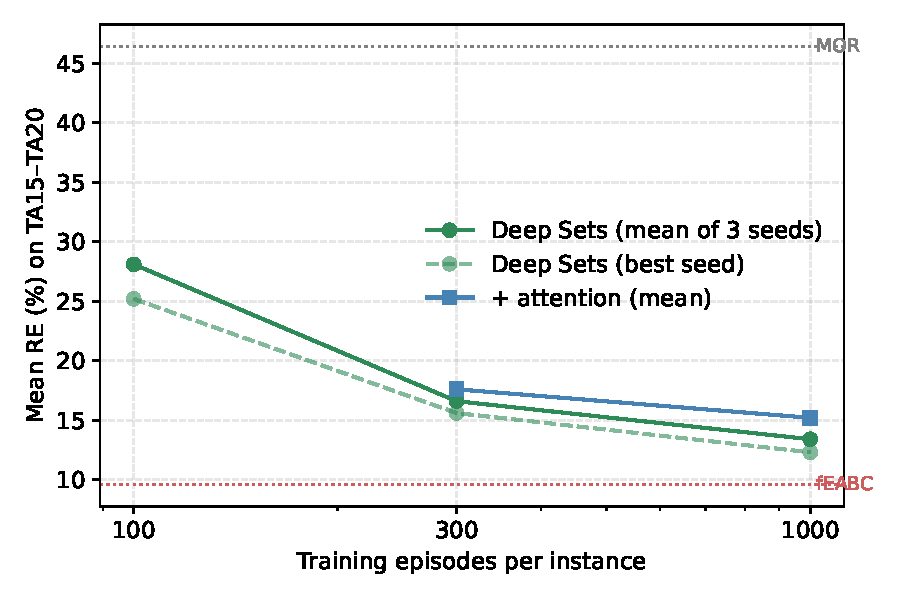
\includegraphics[width=.7\linewidth]{figures/fig_scaling.pdf}
  \caption{Mean RE on the development set versus training episodes per
  instance. Dotted lines: best dispatching rule and published
  metaheuristics (different computational class) as yardsticks.}
  \label{fig:scaling}
\end{figure}

\subsection{Zero-shot cross-size generalization}
\label{sec:results-crosssize}

The size-invariant design allows direct evaluation of the
$20{\times}15$-trained network on any class.
Figure~\ref{fig:crosssize} and Table~\ref{tab:crosssize} report
zero-shot RE on unseen instances of all seven classes: the policy
outperforms MOR on \emph{every} tested instance, with graceful
degradation (best classes: $7$--$10\%$; hardest transfers,
$30{\times}20$ and $50{\times}15$: $24$--$25\%$) and no failure mode up
to $1000$-operation episodes. Notably, transfer quality improves with
in-size training budget (e.g.\ $30{\times}20$: $32.3\%$ with the
$300$-episode checkpoint versus $24.5\%$ with the $1000$-episode one),
i.e.\ the specialist learns structure that is not size-bound.

\begin{table}[t]
\centering\small
\caption{Zero-shot RE (\%) of the $20{\times}15$ specialist (single
network, best-of-64) versus MOR. $\dagger$: $300$-episode checkpoint.}
\label{tab:crosssize}
\begin{tabular}{lcc@{\qquad}lcc}
\toprule
Instance & Policy & MOR & Instance & Policy & MOR \\
\midrule
TA1 ($15{\times}15$) & 14.4 & 29.7 & TA31 ($30{\times}15$) & 13.9 & 34.4 \\
TA2 ($15{\times}15$) & 7.0 & 34.8 & TA41 ($30{\times}20$) & 24.5 & 53.5 \\
TA5 ($15{\times}15$) & 8.7 & 50.7 & TA51 ($50{\times}15$)$^\dagger$ & 25.0 & 38.2 \\
TA21 ($20{\times}20$) & 9.6 & 40.8 & TA61 ($50{\times}20$) & 15.1 & 48.7 \\
TA25 ($20{\times}20$) & 15.9 & 53.2 & & & \\
\bottomrule
\end{tabular}
\end{table}

\begin{figure}[t]
  \centering
  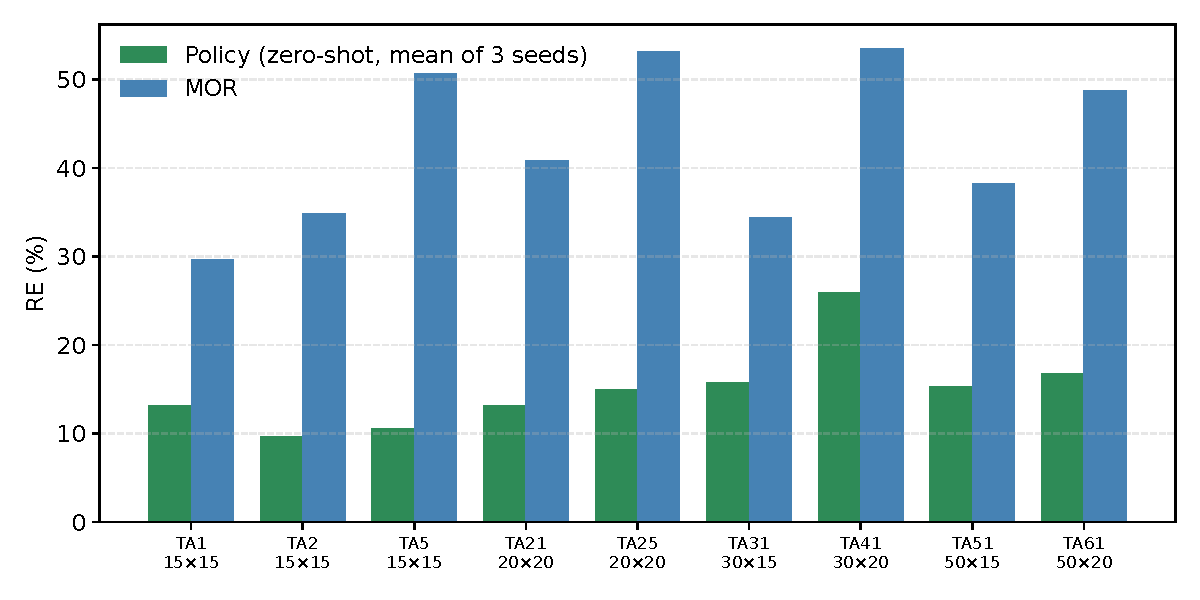
\includegraphics[width=.9\linewidth]{figures/fig_crosssize.pdf}
  \caption{Zero-shot RE by instance across all seven Taillard size
  classes for the $20{\times}15$-trained specialist versus MOR.}
  \label{fig:crosssize}
\end{figure}

\subsection{Ablation: best-of-$N$ inference}
\label{sec:ablations-bon}

Introducing best-of-64 inference (over one greedy rollout) improved the
full-benchmark mean makespan by $3.6\%$, strictly better on 3 of 6
development instances and worse on none, while sharply reducing seed
variance. Diagnostically, before this change the best training
solutions frequently arose in early, exploratory episodes and were
never surpassed by the greedy policy---evidence that the policy's value
concentrates in its sampling distribution.

\subsection{Ablation: attention versus pooling}
\label{sec:ablations-attn}

Two pre-LN self-attention blocks over the candidate embeddings
(identical code path, one flag) were evaluated at both operating points
with paired seeds: $+1.2\%$ mean makespan at $300$ episodes (all six
instances within the noise threshold) and $+1.6\%$ at $1000$ (one
instance significantly worse), at ${\approx}30\%$ higher per-episode
cost (Table~\ref{tab:insize-attn}). At these budgets the pooled context
already conveys the interaction information the policy can exploit;
richer pairwise structure may require larger budgets or instance
distributions to pay off.

\begin{table}[t]
\centering\small
\caption{Attention ablation: mean [best] RE (\%) on the development
set.}
\label{tab:insize-attn}
\begin{tabular}{lcc}
\toprule
Configuration & 300 eps & 1000 eps \\
\midrule
Deep Sets & \textbf{16.4} [15.5] & \textbf{13.4} [12.3] \\
+ attention ($B{=}2$) & 17.5 [16.1] & 15.0 [13.9] \\
\bottomrule
\end{tabular}
\end{table}

\subsection{Ablation: specialist versus multi-size training}
\label{sec:ablations-neg}

Size invariance enables training on mixed size classes, a natural
hypothesis for improving transfer. We trained agents on twelve
instances spanning $15{\times}15$, $20{\times}15$ and $20{\times}20$,
at matched total budget ($3000$ episodes) and at matched
\emph{per-instance} budget ($12{,}000$ episodes), against the
$20{\times}15$ specialist. The specialist won on \emph{all} five common
evaluation instances in both settings---including instances of the size
classes the multi-size agent itself trained on (budget-equalized: $8.7$
vs.\ $9.5$ on $15{\times}15$; $15.9$ vs.\ $18.5$ on $20{\times}20$;
$24.5$ vs.\ $28.3$ on the unseen $30{\times}20$). Per-instance training
depth dominates size diversity, and---contrary to the intuition that
transfer requires diverse training---specialist generalization is the
stronger phenomenon. Earlier development iterations provide the
complementary caution: appending features that are linear combinations
of existing ones, or retrofitting input normalization onto a system
co-adapted to raw scales, degraded performance by $9$--$113\%$;
representation changes must be co-designed with optimization.

\subsection{Positioning and computational cost}
\label{sec:positioning}

Training the final model takes ${\approx}80$ minutes per seed
($4{\times}1000$ episodes) on a commodity CPU; constructing a solution
takes milliseconds (greedy) to a few seconds (best-of-64 on
$50{\times}20$). Raising the inference budget to best-of-$1024$ brings
the full-benchmark mean RE to $12.7\%$ over the 70 instances---ahead of
every deterministic constructive baseline on every instance, within
$2.2$--$4.6$ points of the fEABC 30-run average per class, and behind
tuned tabu search everywhere. The policy's standalone RE ($13.4\%$
in-size; $7$--$25\%$ zero-shot) thus sits between dispatching rules
(${\approx}46\%$) and per-instance metaheuristics
($4$--$10\%$)---establishing, for the IJSP, the computational-class
trade-off documented for the deterministic JSP~\cite{Zhang2020L2D}.

\section{Conclusions and Future Work}
\label{sec:conclusions}

The three questions posed in the introduction now have answers. A
constructive policy trained by PPO on four interval instances beats the
best hand-crafted constructive baselines by a wide margin on its
training class (Q1: $13.4\%$ versus $29.4\%$ for G\&T-MWKR and
${\approx}46\%$ for the best plain rule). Because the representation is
dimensionless and the encoder permutation-invariant, one network serves
the entire benchmark: evaluated zero-shot, it outperforms the best
dispatching rule on every tested instance of all seven size classes
(Q2). And of the standard toolbox, only best-of-$N$ inference paid off
at practical budgets: self-attention did not improve on pooling,
multi-size training lost to the single-size specialist even
budget-equalized, and two independent automatic-configuration campaigns
failed to beat literature-standard hyperparameters at the operating
budget (Q3)---three negative results we document with the same care as
the positive ones.

\paragraph{Limitations.} The benchmark, standard in the IJSP
literature, perturbs crisp instances with symmetric intervals of
bounded relative width; heterogeneous or asymmetric uncertainty, where
worst-case and expected-value criteria diverge more sharply, is
untested. The policy commits to semiactive schedules, so solution
quality is bounded by that space. Results aggregate three training
seeds---enough to report means, bests and seed variance, not formal
significance across seeds. Finally, this paper characterizes the policy
in isolation; a controlled comparison with learned symbolic rules
under matched budgets~\cite{DiazGP2026,Xu2025}, and the use of the
policy's sampling distribution to initialize population-based
search~\cite{DiazTS2026}, are the subject of dedicated ongoing work.

Beyond these, we see two directions: instance distributions with
heterogeneous uncertainty, and curricula or fine-tuning protocols that
exploit size invariance to specialize cheaply on new size classes.

\paragraph{Reproducibility.} Code, benchmark harness, all experiment
records (accepted and rejected), final checkpoints and
figure-generation scripts will be deposited openly; the benchmark
instances are already available~\cite{DiazDataset2026}. \todo{DOI del
dep\'osito propio al enviar}

\paragraph{Funding.} Supported by the Spanish Ministry of Science,
Innovation and Universities (MCIN/AEI/10.13039/501100011033) under
grant PID2022-141746OB-I00.

% NOTA: declaración de uso de IA generativa pendiente de decisión del
% autor antes del envío (política de Springer Nature: en métodos o
% agradecimientos).

\begin{thebibliography}{99}

\bibitem{GareyJohnson1976}
M.~R.~Garey, D.~S.~Johnson, R.~Sethi.
\newblock The complexity of flowshop and jobshop scheduling.
\newblock \textit{Mathematics of Operations Research}, 1(2):117--129, 1976.

\bibitem{GonzalezRodriguez2010}
I.~Gonz\'alez-Rodr\'iguez, C.~R.~Vela, J.~Puente.
\newblock A genetic solution based on lexicographical goal programming
  for a multiobjective job shop with uncertainty.
\newblock \textit{Journal of Intelligent Manufacturing}, 21(1):65--73,
  2010.

\bibitem{Palacios2015}
J.~J.~Palacios, I.~Gonz\'alez-Rodr\'iguez, C.~R.~Vela, J.~Puente.
\newblock Coevolutionary makespan optimisation through different ranking
  methods for the fuzzy flexible job shop.
\newblock \textit{Fuzzy Sets and Systems}, 278:81--97, 2015.

\bibitem{Lei2012}
D.~Lei.
\newblock Population-based neighborhood search for job shop scheduling
  with interval processing time.
\newblock \textit{Computers \& Industrial Engineering}, 62(4):1200--1208,
  2012.

\bibitem{DiazGA2020}
H.~D\'iaz, I.~Gonz\'alez-Rodr\'iguez, J.~J.~Palacios, I.~D\'iaz,
C.~R.~Vela.
\newblock A genetic approach to the job shop scheduling problem with
  interval uncertainty.
\newblock In \textit{Information Processing and Management of
  Uncertainty in Knowledge-Based Systems (IPMU)}, pages 663--676.
  Springer, 2020.

\bibitem{DiazTardiness2022}
H.~D\'iaz, J.~J.~Palacios, I.~D\'iaz, C.~R.~Vela,
I.~Gonz\'alez-Rodr\'iguez.
\newblock Robust schedules for tardiness optimization in job shop with
  interval uncertainty.
\newblock \textit{Logic Journal of the IGPL}, 31(2):240--254, 2022.

\bibitem{Sotskov2020}
Y.~N.~Sotskov, N.~M.~Matsveichuk, V.~D.~Hatsura.
\newblock Schedule execution for two-machine job-shop to minimize
  makespan with uncertain processing times.
\newblock \textit{Mathematics}, 8(8):1314, 2020.

\bibitem{Zheng2024}
P.~Zheng, S.~Xiao, P.~Zhang, Y.~Lv.
\newblock A two-individual-based evolutionary algorithm for flexible
  assembly job shop scheduling problem with uncertain interval
  processing times.
\newblock \textit{Applied Sciences}, 14(22):10304, 2024.

\bibitem{DiazFEABC2023}
H.~D\'iaz, J.~J.~Palacios, I.~Gonz\'alez-Rodr\'iguez, C.~R.~Vela.
\newblock Fast elitist {ABC} for makespan optimisation in interval {JSP}.
\newblock \textit{Natural Computing}, 22(4):645--657, 2023.

\bibitem{DiazICAE2023}
H.~D\'iaz, J.~J.~Palacios, I.~Gonz\'alez-Rodr\'iguez, C.~R.~Vela.
\newblock An elitist seasonal artificial bee colony algorithm for the
  interval job shop.
\newblock \textit{Integrated Computer-Aided Engineering}, 30(3):223--242,
  2023.

\bibitem{DiazTS2026}
H.~D\'iaz et al.
\newblock Neighbourhood structures and ranking operators for the interval
  job shop scheduling problem.
\newblock Under review, 2026.

\bibitem{DiazGP2026}
H.~D\'iaz Rodr\'iguez.
\newblock Genetic programming hyper-heuristics for the job shop
  scheduling problem with interval durations: robustness-aware
  interpretable rules that generalize across instance sizes.
\newblock Under review, 2026.

\bibitem{DiazDataset2026}
H.~D\'iaz Rodr\'iguez.
\newblock Genetic programming dispatching rules for the interval job
  shop: instances, evolved rules, results and code.
\newblock Zenodo, 2026. \texttt{doi:10.5281/zenodo.21716972}.

\bibitem{Taillard1993}
E.~Taillard.
\newblock Benchmarks for basic scheduling problems.
\newblock \textit{European Journal of Operational Research},
  64(2):278--285, 1993.

\bibitem{Xu2025}
M.~Xu, Y.~Mei, F.~Zhang, M.~Zhang.
\newblock Learn to optimise for job shop scheduling: a survey with
  comparison between genetic programming and reinforcement learning.
\newblock \textit{Artificial Intelligence Review}, 58:160, 2025.

\bibitem{Vinyals2015}
O.~Vinyals, M.~Fortunato, N.~Jaitly.
\newblock Pointer networks.
\newblock \textit{NeurIPS}, 2015.

\bibitem{Bello2016}
I.~Bello, H.~Pham, Q.~V.~Le, M.~Norouzi, S.~Bengio.
\newblock Neural combinatorial optimization with reinforcement learning.
\newblock \textit{arXiv:1611.09940}, 2016.

\bibitem{Nazari2018}
M.~Nazari, A.~Oroojlooy, L.~Snyder, M.~Tak\'a\v{c}.
\newblock Reinforcement learning for solving the vehicle routing problem.
\newblock \textit{NeurIPS}, 2018.

\bibitem{Kool2019}
W.~Kool, H.~van Hoof, M.~Welling.
\newblock Attention, learn to solve routing problems!
\newblock \textit{ICLR}, 2019.

\bibitem{Zhang2020L2D}
C.~Zhang, W.~Song, Z.~Cao, J.~Zhang, P.~S.~Tan, C.~Xu.
\newblock Learning to dispatch for job shop scheduling via deep
  reinforcement learning.
\newblock \textit{NeurIPS}, 2020.

\bibitem{Park2021GNN}
J.~Park, J.~Chun, S.~H.~Kim, Y.~Kim, J.~Park.
\newblock Learning to schedule job-shop problems: representation and
  policy learning using graph neural network and reinforcement learning.
\newblock \textit{International Journal of Production Research},
  59(11):3360--3377, 2021.

\bibitem{Tassel2021}
P.~Tassel, M.~Gebser, K.~Schekotihin.
\newblock A reinforcement learning environment for job-shop scheduling.
\newblock \textit{arXiv:2104.03760}, 2021.

\bibitem{Zaheer2017}
M.~Zaheer, S.~Kottur, S.~Ravanbakhsh, B.~P\'oczos, R.~Salakhutdinov,
A.~Smola.
\newblock Deep sets.
\newblock \textit{NeurIPS}, 2017.

\bibitem{Schulman2017}
J.~Schulman, F.~Wolski, P.~Dhariwal, A.~Radford, O.~Klimov.
\newblock Proximal policy optimization algorithms.
\newblock \textit{arXiv:1707.06347}, 2017.

\bibitem{GifflerThompson1960}
B.~Giffler, G.~L.~Thompson.
\newblock Algorithms for solving production-scheduling problems.
\newblock \textit{Operations Research}, 8(4):487--503, 1960.

\bibitem{Branke2016}
J.~Branke, S.~Nguyen, C.~W.~Pickardt, M.~Zhang.
\newblock Automated design of production scheduling heuristics: a review.
\newblock \textit{IEEE Transactions on Evolutionary Computation},
  20(1):110--124, 2016.

\bibitem{Nguyen2017}
S.~Nguyen, Y.~Mei, M.~Zhang.
\newblock Genetic programming for production scheduling: a survey with a
  unified framework.
\newblock \textit{Complex \& Intelligent Systems}, 3(1):41--66, 2017.

\bibitem{LopezIbanez2016}
M.~L\'opez-Ib\'a\~nez, J.~Dubois-Lacoste, L.~P\'erez~C\'aceres,
M.~Birattari, T.~St\"utzle.
\newblock The irace package: Iterated racing for automatic algorithm
  configuration.
\newblock \textit{Operations Research Perspectives}, 3:43--58, 2016.

\end{thebibliography}

\end{document}
